\documentclass{article}

\usepackage[utf8]{inputenc}
\usepackage{enumitem}
\usepackage{multirow}
\usepackage{xcolor}
\usepackage[T1]{fontenc}
% \usepackage[french]{babel}
\usepackage{hyperref}
\usepackage{amssymb}
\usepackage{mathtools}
\usepackage{ntheorem}
\usepackage{amsmath}
\usepackage{amssymb}
\usepackage[ a4paper, hmargin={2cm, 2cm}, vmargin={3cm, 3cm}]{geometry}
\usepackage{capt-of}
\usepackage{multicol}
\usepackage{mathpartir}

\usepackage[braket, qm]{qcircuit}
\usepackage{graphicx}

\usepackage{tikz}
\usetikzlibrary{angles,quotes, 3d}

\usepackage{hyperref}
\hypersetup{
    colorlinks,
    citecolor=black,
    filecolor=black,
    linkcolor=blue,
    urlcolor=blue
}

\usepackage{xcolor}

\definecolor{codegreen}{rgb}{0,0.6,0}
\definecolor{codegray}{rgb}{0.5,0.5,0.5}
\definecolor{codepurple}{rgb}{0.58,0,0.82}

\usepackage{listings}
\lstdefinestyle{mystyle}{
    commentstyle=\color{codegreen},
    keywordstyle=\color{magenta},
    numberstyle=\tiny\color{codegray},
    stringstyle=\color{codepurple},
    basicstyle=\ttfamily\footnotesize,
    breakatwhitespace=false,
    breaklines=true,
    captionpos=b,
    keepspaces=true,
    numbers=left,
    numbersep=5pt,
    showspaces=false,
    showstringspaces=false,
    showtabs=false,
    tabsize=2
}
\lstset{style=mystyle}

\theoremstyle{plain}
\theorembodyfont{\normalfont}
\theoremseparator{~--}
\newtheorem*{proof}{Proof}
\newtheorem*{exam}{Example}
\renewcommand\qedsymbol{$\square$}

\newtheorem*{defi}{Definition}
\newtheorem{exo}{Exercise}[section]
\newtheorem{ans}{Answer}[section]
\newtheorem*{lemma}{Lemma}%[section]

\newcommand{\toto}{\twoheadrightarrow}

\newcommand{\rbeta}{\to_\beta}
\newcommand{\rsbeta}{\to_\beta^*}

\newcommand{\Mlambda}{{\underline \Lambda}}
\newcommand{\mlambda}{{\underline \lambda}}
\newcommand{\mbeta}{{\underline \beta}}
\date{}
\newcommand{\tombeta}{\to_\mbeta}
\newcommand{\tosmbeta}{\to_\mbeta^*}

\title{$\lambda$-calculus}
\author{Valeran MAYTIE}

\begin{document}
  \maketitle

  \lemma \label{lemma:bar-phi}
  $\forall t, |t| \rsbeta \varphi(t)$

  \begin{center}
    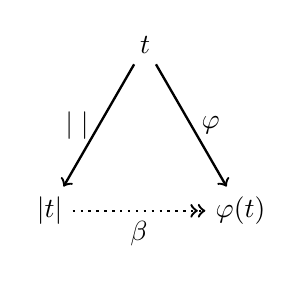
\begin{tikzpicture}[line width=0.3mm, scale=1.4]
    \node(t) at (90:1) {$t$};
    \node(bt) at (210:1) {$|t|$};
    \node(pt) at (330:1) {$\varphi(t)$};

    \draw[->] (t) edge node[left] {$|\;|$} (bt)
              (t) edge node[right] {$\varphi$} (pt);
    \draw[->>, dotted] (bt) edge node[below] {$\beta$} (pt);
  \end{tikzpicture}
  \end{center}
  \textit{Proof}: We will show our property by induction on the term $t$.
  \begin{itemize}
    \item Case $t = x$, $|x| = x = \varphi(x)$, so we have $|t| \to_\beta^0
      \varphi(t)$.
    \item Case $t = \lambda x. t_0$, by the induction hypothesis we know that
      $|t_0| \rsbeta \varphi(t_0)$.
      \begin{align*}
        |(\lambda x. t_0)| &= \lambda x. |t_0| \\
        &\rsbeta \lambda x. \varphi(t_0) & \text{By induction hypothesis} \\
        &= \varphi(\lambda x. t_0)
      \end{align*}

    \item Case $t = \mlambda x. t_0$, by the induction hypothesis we know that
      $|t_0| \rsbeta \varphi(t_0)$.
      \begin{align*}
        |(\mlambda x. t_0)| &= \lambda x. |t_0| \\
        &\rsbeta \lambda x. \varphi(t_0) & \text{By induction hypothesis} \\
        &= \varphi(\mlambda x. t_0)
      \end{align*}

    \item Case $t = t_1\; t_2$ where $t_1 \not = \mlambda x. t_0$,
      by the induction hypothesis we know that
      $|t_1| \rsbeta \varphi(t_1)$ and $|t_2| \rsbeta \varphi(t_2)$.
      \begin{align*}
        |t_1\;t_2| &= |t_1|\;|t_2| \\
        &\rsbeta \varphi(t_1)\;\varphi(t_2) & \text{By induction hypothesis} \\
        &= \varphi(t_1\;t_2)
      \end{align*}

    \item Case $t=(\mlambda x. t_0)\;t_1$, by the induction hypothesis we know that
      $|t_0| \rsbeta \varphi(t_0)$ and $|t_1| \rsbeta \varphi(t_1)$.

        \begin{align*}
          |(\mlambda x. t_0)\;t_1| &= (\lambda x. |t_0|)\;|t_1| \\
            &\rsbeta (\lambda x. \varphi(t_0))\;\varphi(t_1) & \text{By
            induction hypothesis}\\
            &\to \varphi(t_0)\{x \leftarrow \varphi(t_1)\} \\
            &=\varphi((\mlambda x. t_0)\;t_1)
        \end{align*}

  \end{itemize}

  \qedsymbol
\end{document}
